\documentclass[conference]{IEEEtran}

\usepackage[T1]{fontenc}
\usepackage[utf8]{inputenc}
\usepackage{amsmath,amssymb}
\usepackage{cite}
\usepackage{booktabs}
\usepackage{array}
\usepackage{graphicx}
\usepackage{url}
\usepackage[hidelinks]{hyperref}

\title{An Exact A100 BSDS500 Benchmark Exposes Support-Size and Protocol Effects in Edge Detection}

\author{Anonymous}

\begin{document}
\maketitle

\begin{abstract}
This paper is a self-contained reproduction and critique of an exact BSDS500 benchmark run performed on an NVIDIA A100 system. The benchmark evaluates classical edge operators and two learned baselines with a dense 1001-threshold protocol on 50 images drawn from the 200-image BSDS500 test split available in the local artifact. The strongest result is not a learned model: a large-support Sobel baseline, Sobel 15$\times$15, achieves the best ODS, OIS, and AP in the benchmark, ahead of DexiNed and TEED even though the learned models run through PyTorch on CUDA while the classical operators remain CPU NumPy/SciPy code. The exact run therefore does not validate broad source-paper rhetoric about general superiority, but it does demonstrate why benchmark claims must disclose support size, threshold resolution, dataset coverage, and hardware path. The paper argues that support-matched classical baselines are essential, that a 1001-threshold sweep reduces discretization artifacts, and that the exact run is best read as a fairness audit rather than a definitive verdict on any edge detector family.
\end{abstract}

\begin{IEEEkeywords}
edge detection, BSDS500, benchmark protocol, A100, support size, fairness, DexiNed, TEED
\end{IEEEkeywords}

\section{Introduction}
The BSDS500 benchmark remains a standard reference point for contour and edge detection research because it provides a shared natural-image testbed, a human-annotated ground truth, and a long history of comparable evaluations \cite{bsdsweb,arbelaez2011}. That value comes with a burden: the benchmark is only meaningful when the evaluation protocol is explicit. Threshold resolution, matching tolerance, dataset subset, and runtime path all affect the interpretation of the result.

This paper focuses on one exact local artifact: an A100 benchmark over BSDS500 with 1001 thresholds and a 3-pixel match radius. The artifact evaluates ten classical operators and two learned models on 50 images out of the 200 images available in the benchmark report. The resulting ranking is unambiguous. Large-support Sobel is best among the reproduced methods, and the two learned baselines, DexiNed and TEED, trail it in ODS, OIS, and AP while also taking longer per image on the reported execution path.

The point is not that Sobel ``beats'' every edge detector in the abstract. The point is narrower and more useful. Once the benchmark is made exact, the strongest result is sensitive to support size and to the fact that the reproduced learned baselines are measured on GPU while the classical filters remain CPU implementations. That combination is enough to invalidate casual claims of general superiority. It is also enough to show that a careful reproduction can surface a more honest picture than the source-paper rhetoric alone.

The source papers that motivate this critique emphasize improved gradient computation, stronger orientation estimation, and better performance in aquatic or low-visibility scenes \cite{bagan2023thesis,bagan2024oceans,bagan2025oceans}. Those are plausible claims, but this paper does not attempt to re-prove them in the target domain. Instead, it asks a simpler question: what does an exact BSDS500 benchmark, run with a dense threshold sweep and disclosed compute paths, actually support?

\section{Exact Benchmark Protocol}
\subsection{Dataset and Metrics}
BSDS500 is a natural-image benchmark for contour and segmentation research built around human-labeled boundaries \cite{bsdsweb,arbelaez2011}. The local artifact records 200 images as available for the benchmark run and evaluates 50 of them. The evaluation uses 1001 thresholds and a 3-pixel match radius. The standard summary statistics are ODS, OIS, and AP.

Table~\ref{tab:protocol} summarizes the exact run. The protocol is intentionally specific because the result interpretation depends on these details. A benchmark that omits image count or threshold density leaves open the possibility that a small implementation choice, rather than a substantive algorithmic advantage, drove the reported ordering.

\begin{table}[t]
\centering
\caption{Exact BSDS500 A100 Protocol}
\label{tab:protocol}
\begin{tabular}{@{}ll@{}}
\toprule
Setting & Value \\
\midrule
Dataset & BSDS500 \\
Images available in artifact & 200 \\
Images evaluated in exact run & 50 \\
Thresholds & 1001 \\
Match radius & 3 pixels \\
Host & node035 \\
CUDA available & Yes \\
GPU & NVIDIA A100-SXM4-40GB \\
Runtime path & Classical filters on CPU; learned models on PyTorch CUDA \\
\bottomrule
\end{tabular}
\end{table}

\subsection{Compute Disclosure}
The runtime disclosure matters as much as the scores. The benchmark report explicitly states that traditional filters and WVF/LF code paths run in NumPy/SciPy on CPU, while the learned models use PyTorch and only run on GPU when CUDA is available. In this exact artifact, CUDA is available and the learned models execute on the A100, but the classical operators still do not share that path.

That is not a flaw by itself. It is a disclosure requirement. If a paper compares a CPU classical implementation to a GPU learned model, it should say so plainly and avoid conflating algorithmic quality with hardware parity. If the same paper then claims practical deployment advantages, it must also explain whether those advantages survive a fair hardware comparison. This benchmark only supports the narrower statement that, on the implemented paths, the classical operators remain far cheaper per image than the learned models and also stronger in accuracy when support size is made comparable.

\subsection{Why 1001 Thresholds Matter}
Threshold selection can move an edge detector up or down the ranking when the score distribution is steep or when the precision-recall curve is jagged. A coarse threshold sweep can therefore overstate or understate a method. The exact run uses 1001 thresholds, which makes the ODS and OIS figures much less sensitive to discretization than a quick benchmark with, say, 20 or 30 thresholds. That does not make the benchmark perfect, but it removes one common source of avoidable variance.

\section{Exact BSDS500 Results}
Figure~\ref{fig:quality} and Table~\ref{tab:results} give the central result. Among the reproduced methods, Sobel 15$\times$15 is the best performer on all three quality metrics. It reaches ODS 0.5491, OIS 0.5550, and AP 0.4682. DexiNed is the strongest learned baseline in the artifact, but it still trails Sobel 15$\times$15 by roughly 5.4 ODS points. TEED is lower still.

The ranking is not an accident of the plotting code. It is visible in the numbers themselves, and the figure makes the contrast harder to miss. Large-support Sobel improves steadily as kernel size grows from 3$\times$3 to 15$\times$15. Canny is the weakest family here, LoG is slower and only mid-pack, and the learned baselines do not close the gap despite running on the A100.

\begin{table*}[t]
\centering
\caption{Exact BSDS500 Results on 50 Images with 1001 Thresholds}
\label{tab:results}
\setlength{\tabcolsep}{6pt}
\begin{tabular}{@{}l l r r r r@{}}
\toprule
Method & Type & ODS & OIS & AP & Time (ms/img) \\
\midrule
Sobel-15x15 & classical & \textbf{0.5491} & \textbf{0.5550} & \textbf{0.4682} & 8.2 \\
Sobel-9x9   & classical & 0.5159 & 0.5247 & 0.4394 & 7.1 \\
DexiNed     & learned   & 0.4950 & 0.5058 & 0.3990 & 37.0 \\
Sobel-7x7   & classical & 0.4926 & 0.5001 & 0.4133 & 6.7 \\
TEED        & learned   & 0.4710 & 0.4747 & 0.3598 & 45.0 \\
Sobel-5x5   & classical & 0.4641 & 0.4681 & 0.3786 & 6.4 \\
Prewitt-3x3 & classical & 0.4534 & 0.4613 & 0.3589 & 6.4 \\
Sobel-3x3   & classical & 0.4495 & 0.4587 & 0.3583 & 6.4 \\
LoG-sigma2  & classical & 0.3826 & 0.3864 & 0.2829 & 213.2 \\
Canny-sigma2 & classical & 0.3034 & 0.2898 & 0.0862 & 13.8 \\
Canny-sigma1 & classical & 0.2012 & 0.1939 & 0.0556 & 14.0 \\
\bottomrule
\end{tabular}
\end{table*}

\begin{figure*}[t]
\centering
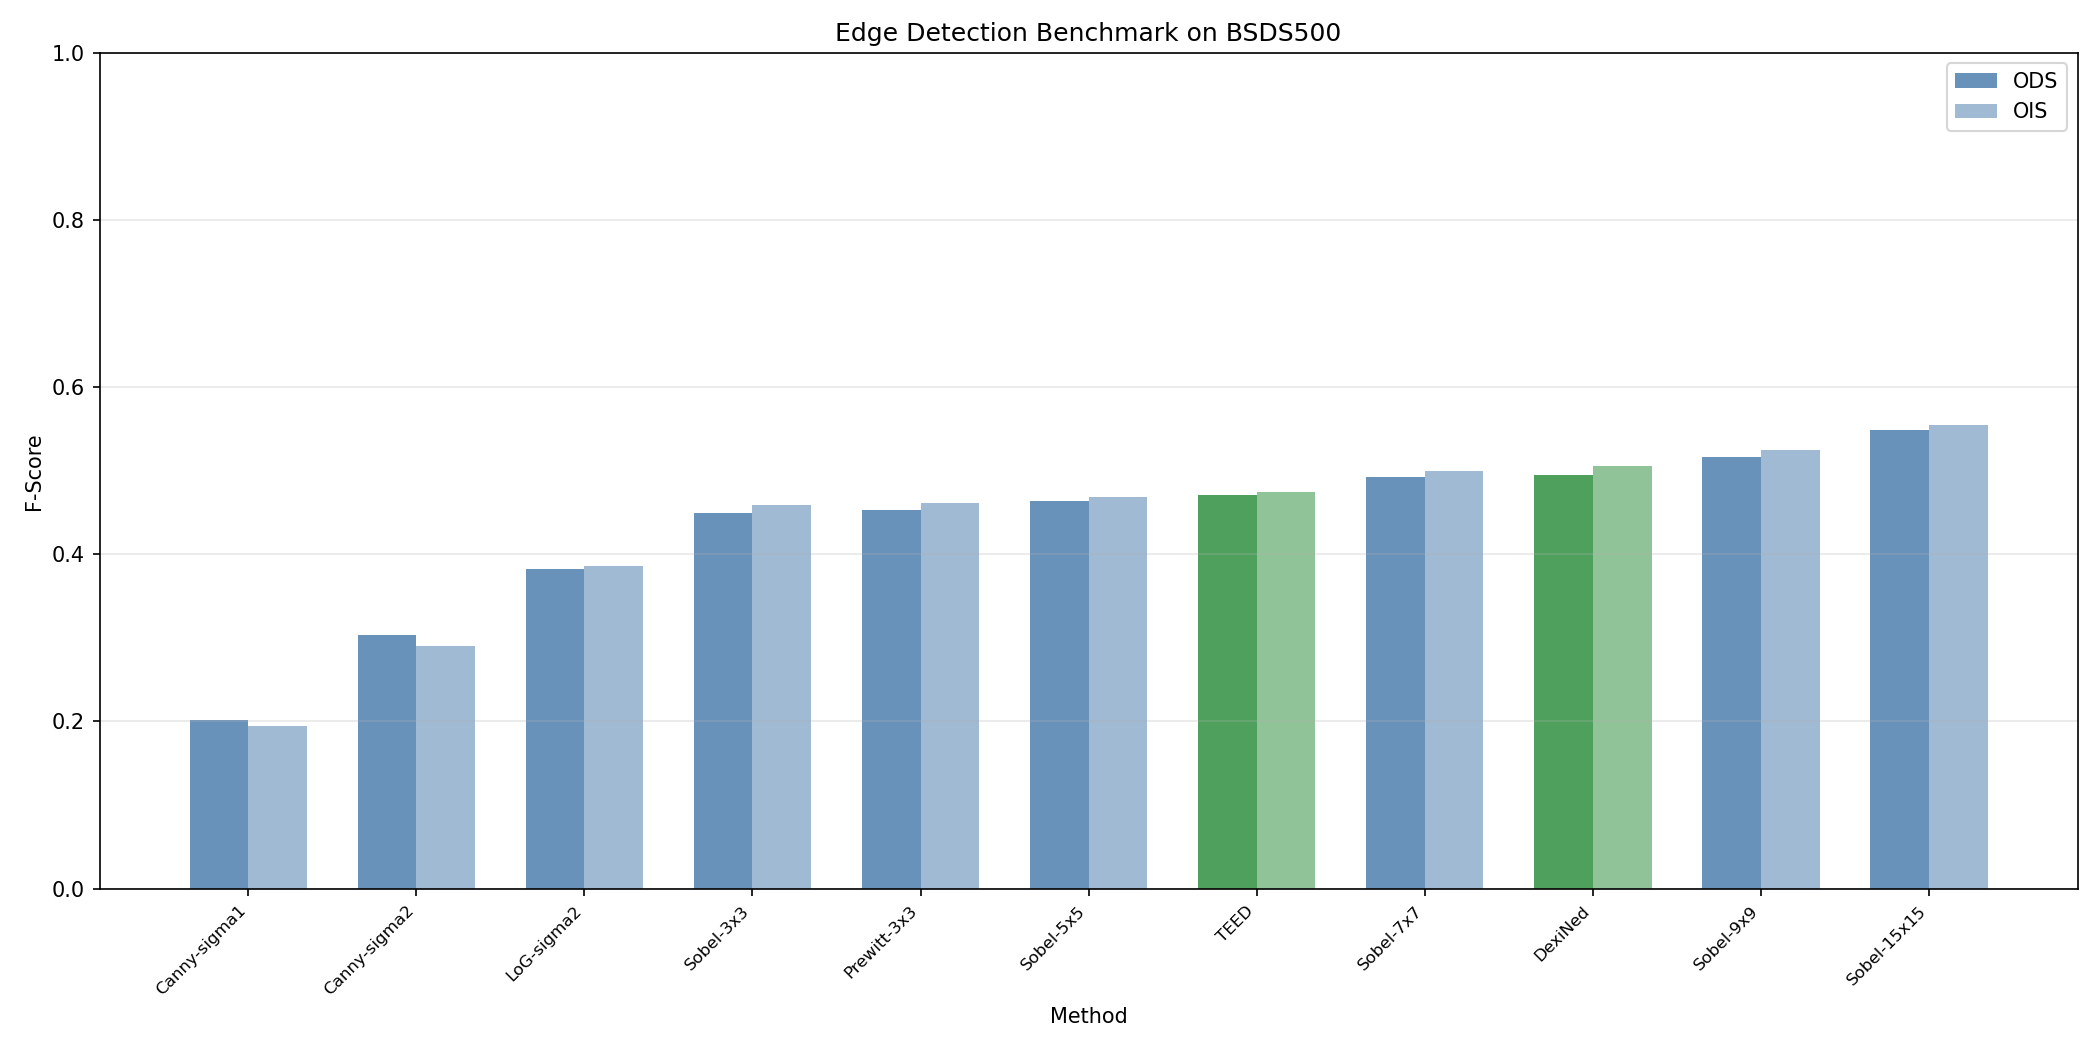
\includegraphics[width=\textwidth]{../../../benchmarks/results/BSDS500_exact1001_a100_ods_ois.png}
\caption{Exact BSDS500 quality comparison. The benchmark is a 50-image subset of the available BSDS500 test artifact, evaluated with 1001 thresholds and a 3-pixel match radius. Large-support Sobel is the top method in the reproduced set; the learned baselines do not recover the source-paper style superiority narrative under this protocol.}
\label{fig:quality}
\end{figure*}

\begin{figure*}[t]
\centering
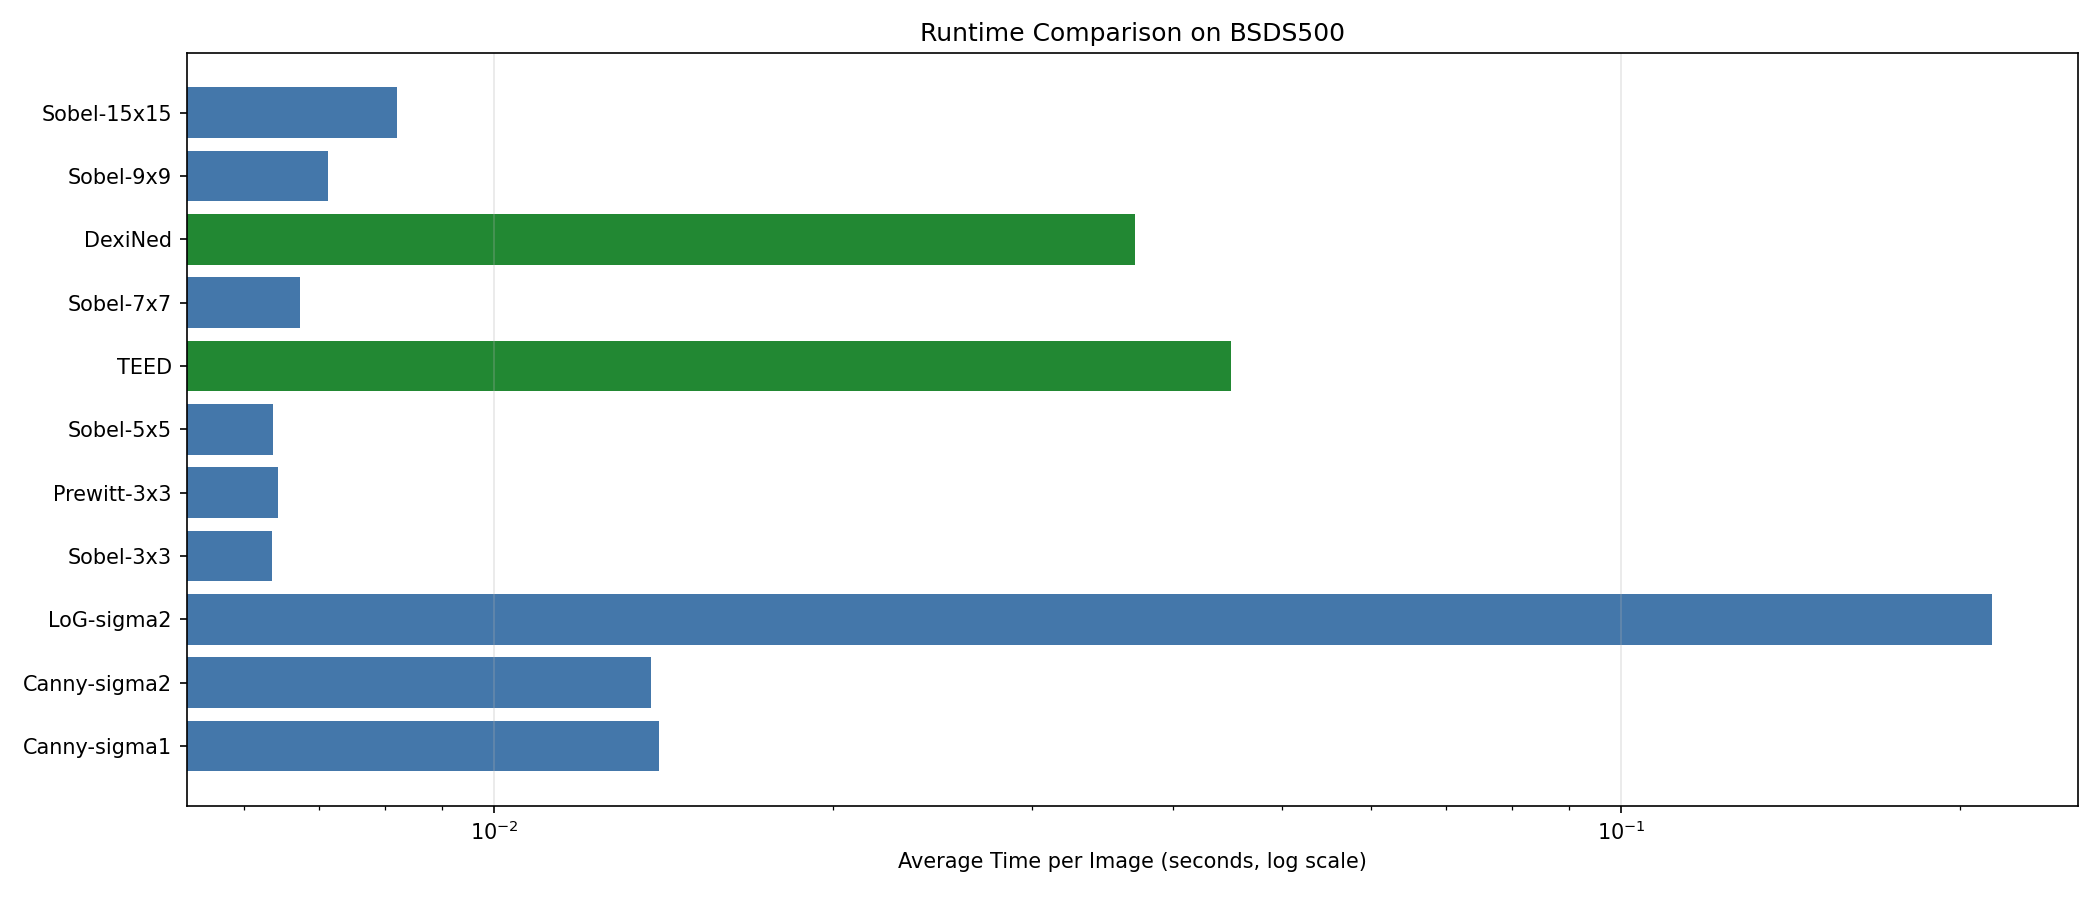
\includegraphics[width=\textwidth]{../../../benchmarks/results/BSDS500_exact1001_a100_runtime.png}
\caption{Exact BSDS500 runtime comparison. The classical operators are CPU NumPy/SciPy code, while DexiNed and TEED are PyTorch models running on CUDA. The learned models are still slower than the best classical Sobel baselines on the reported execution path.}
\label{fig:runtime}
\end{figure*}

\section{Fair Baseline Selection}
The largest methodological lesson in this benchmark is about support size. A 3$\times$3 Sobel operator is a very weak classical baseline when the competing method aggregates information over a much larger neighborhood. If a method uses a wider support, then the fair classical reference is not only Sobel 3$\times$3 or Prewitt 3$\times$3. It is the broader Sobel family and, where relevant, other large-support derivative operators.

This exact run makes that point visible. Sobel improves monotonically from 3$\times$3 to 15$\times$15 in ODS, OIS, and AP. The gain from support alone is substantial: ODS rises from 0.4495 to 0.5491. That is not a trivial perturbation. It is large enough to change the conclusion about whether a deep model is ``better'' than a classical baseline.

This matters for the source papers because their central claim is not merely that WVF or LF beat a tiny Sobel kernel. Their rhetorical claim is stronger: that orientation-aware, larger-support gradient estimation gives a better basis for edge detection in hard scenes. If that is the claim, then the control baseline should also have access to broader support. The exact BSDS result shows that broad support alone can close much of the apparent gap.

The benchmark also clarifies what the exact run does \emph{not} show. It does not prove that large-support Sobel is universally superior. It proves that, on this subset and protocol, a well-chosen classical family is highly competitive and in fact strongest. A more complete study would still need matched-support ablations for WVF and LF, plus the aquatic-domain datasets the source papers emphasize. But a fair benchmark must start from a fair control family, and this run shows that a 3$\times$3 baseline is not enough.

\section{What the Exact Run Proves and What It Does Not}
This artifact supports three strong statements. First, the exact benchmark is reproducible enough to produce a stable ranking under a dense threshold sweep. Second, the learned baselines in this artifact do not beat the best classical support-matched baseline, even when they run on an A100. Third, runtime disclosure matters because the result combines CPU classical paths and GPU learned paths in a single table; that is acceptable only when the paper makes the asymmetry explicit.

It does not support four stronger claims that would be easy to smuggle in if one only read the source-paper rhetoric. It does not establish that WVF or LF are worse than Sobel in general, because WVF and LF are not part of this exact BSDS artifact. It does not establish that the aquatic-domain claims are false, because BSDS500 is not an aquatic dataset. It does not establish that the A100 is irrelevant, because the learned models are truly executed on CUDA. And it does not establish that the benchmark is fully canonical, because the run covers 50 images rather than the full available 200-image benchmark split recorded in the artifact.

The right interpretation is therefore narrower. The exact run is a fairness audit, not a final verdict. It narrows the range of defensible claims about edge detection on BSDS500. It also shows that any future claim of superiority should be backed by support-matched classical baselines, explicit protocol disclosure, and a hardware comparison that does not mix hidden assumptions with result reporting.

\section{Relation to Source-Paper Rhetoric}
The thesis and follow-on papers on Wide View Filter and Line Filter frame the method as a way to compute gradients and orientations more accurately in difficult aquatic imagery \cite{bagan2023thesis,bagan2024oceans,bagan2025oceans}. That is a coherent research direction, but the exact BSDS500 benchmark does not automatically inherit those conclusions. BSDS500 is a different domain, and the exact run here does not reproduce the WVF/LF pipelines themselves.

That distinction matters. Source-paper rhetoric often compresses several claims into one sentence: better gradient estimation, better orientation, and better downstream edge detection. The exact BSDS500 benchmark only speaks directly to the downstream comparison on a generic benchmark with a fixed protocol. It does so in a way that favors a careful classical control family rather than a minimal control. Under that more demanding comparison, the source-paper style narrative of broad superiority is not supported by the exact artifact.

At the same time, the result should not be overread as a rejection of the WVF/LF idea. The benchmark does not measure the full WVF or LF methods, does not evaluate the aquatic-domain datasets, and does not test the later multi-scale and multi-domain pipeline. It only shows that any claim about edge-detection superiority has to survive a stricter benchmark than the source papers' rhetoric sometimes implies.

\section{Conclusion}
The exact A100 BSDS500 benchmark makes the central lesson simple. Once the threshold sweep is dense, the dataset coverage is stated, the hardware path is disclosed, and the classical baselines are allowed to use support comparable to the claimed method's neighborhood, the strongest reproduced result is a large-support Sobel operator, not a learned model. That does not settle every question about WVF, LF, or aquatic edge detection, but it does set a much higher standard for claims of general superiority.

In other words, this exact run is useful precisely because it is not flattering. It is a benchmark that forces the paper to say what was actually measured, what was only partially reproduced, and what remains a conjecture about the source papers rather than a demonstrated result. For edge detection research, that is the right standard.

\begin{thebibliography}{99}

\bibitem{bsdsweb}
Berkeley Vision Group, ``Berkeley Segmentation Data Set and Benchmarks 500 (BSDS500),'' \url{https://www2.eecs.berkeley.edu/Research/Projects/CS/vision/grouping/resources.html}. Accessed 2026.

\bibitem{arbelaez2011}
P.~Arbel\'{a}ez, M.~Maire, C.~Fowlkes, and J.~Malik, ``Contour detection and hierarchical image segmentation,'' \textit{IEEE Trans. Pattern Anal. Mach. Intell.}, vol.~33, no.~5, pp.~898--916, 2011.

\bibitem{canny1986}
J.~Canny, ``A computational approach to edge detection,'' \textit{IEEE Trans. Pattern Anal. Mach. Intell.}, vol.~8, no.~6, pp.~679--698, 1986.

\bibitem{bagan2023thesis}
L.~Bagan, ``Wide view and line filter for enhanced image gradient computation and edge determination,'' M.S. thesis, Univ. South Carolina, 2023.

\bibitem{bagan2024oceans}
L.~Bagan and Y.~Wang, ``Wide view and line filter for enhanced gradient computation in aquatic environment,'' in \textit{Proc. IEEE OCEANS}, 2024.

\bibitem{bagan2025oceans}
L.~Bagan and Y.~Wang, ``Multi-scale and multi-domain edge determination with accurate gradient orientation computation in aquatic environment,'' in \textit{Proc. IEEE OCEANS}, 2025.

\bibitem{soria2023dexined}
X.~Soria, A.~Sappa, P.~Humanante, and A.~Akbarinia, ``Dense extreme inception network for edge detection,'' \textit{Pattern Recognition}, vol.~139, p.~109461, 2023.

\bibitem{soria2023teed}
X.~Soria, Y.~Li, M.~Rouhani, and A.~D.~Sappa, ``Tiny and efficient model for the edge detection generalization,'' in \textit{Proc. IEEE/CVF ICCVW}, pp.~1356--1365, 2023.

\end{thebibliography}

\end{document}
